\documentclass[a4paper,10pt]{article}
\usepackage[utf8]{inputenc}
\usepackage[english,russian]{babel}
\usepackage{amsmath}
\usepackage[pdftex]{graphicx}
\usepackage{epstopdf}
\usepackage{a4wide}
\usepackage{hyperref}

%opening
\title{Инфракрасные области поглощения межзвездной пыли}
\author{Артамонов Алексей}
\bibliographystyle{plain}
\begin{document}
\maketitle


\section{Введение}
\par Химичкский состав межзвездных пылинок может быть определен
путем изучения инфракрасных полос, наблюдаемых в спектрах звезд и 
протозвездных объектов. При этом исследуют профили полос и поляризацию в них.
Инфракрасные полосы несут также информацию о размере, структуре 
и форме пылинок.\\
\par Оптическая толщина в полосе и поляризация в ней определяются свойствами пылинок,
их лучевой концентрацие	 $N_d$, а так же степенью и направлением их ориентации.
Для неполяризованного падающего излучения они равны:

$$\tau(\lambda) = N_d(r)\frac{1}{2}[C^{TM}_{ext}(m_{\lambda,2\pi r_V/\lambda,\alpha})+C^{TE}_{ext}(m_{\lambda,2\pi r_V/\lambda,\alpha})],$$
$$P(\lambda) = N_d(r)\frac{1}{2}[C^{TM}_{ext}(m_{\lambda,2\pi r_V/\lambda,\alpha})-C^{TE}_{ext}(m_{\lambda,2\pi r_V/\lambda,\alpha})].$$

Здесь $r_V$ --- характерный размер несферической пылинки (ее объем равен объему шара с радиусом $r_V$
),$C^{TM,TE}_{ext} = C^{TM,TE}_{abs}+C^{TM,TE}_{sca}$ --- фактор эффективности ослабления для двух
случаев поляризации падающего излучения, $\alpha$ --- угол падения излучения 
(для сфероидов угол между волновым вектором и осью вращения частицы $0^{o}\geq\alpha\geq90^{o}$),
$m_\lambda = n - ki$ --- комплексный показатель преломления вещества пылинки.
\\
\\
Итого сделано:\\
1. Проведены расчеты нормированных зависимостей $\tau{\lambda}/\tau(3\mu m)$ и $P(\lambda/\tau(\lambda))$ 
в диапозоне длин волн 3 -- 25 $\mu m$, включающим в себя ледяную ($3\mu m$) и силикатные полосы астрономического силиката.
При этом использовались данные:
\par Показатели преломления для льда и силикатов(База JPDOC: astro.spbu.ru/JPDOC);
\par Квазистатическое приближение для сфероидальных частиц с оболочкой( вернее сое ее представление ), 
описанное формулами в главе 'Рабочие формулы'
\\
\par Были рассмотрены вытянутые частицы с разными отношениями полуосей и разными размерами.
\newpage
\section{Рабочие формулы и константы}
Ряд формул с помощью которых производились вычисления \\

$\lambda\text{ -- длина волны излучения}\nonumber \\$\\
$d\text{ --- фокусное расстояние сфероида}\nonumber $\\
$c = 2\pi/\lambda\cdotp$ --- размерный параметр\\
$a_{ice},b_{ice}$ --- большая и малая полуось льдинки\\
$a_{sil},b_{sil}$ --- большая и малая полуось силиката\\
$\alpha$ --- угол между осью вращения и волновым вектором приходящего излучения\\
$m$ --- коэффициент приломления ($\varepsilon = m^2$)\\
$Q_{ext}$ --- ослабление света\\
$Q_{abs}$ --- истинное поглощение света\\
$Q_{sca}$ --- рассеивание света\\
\~{a}$_j$ --- степень поляризации\\
$f = 1 ? prolate : -1$ \\
\~{f}$ = V_{core}/V_{total}$ --- отношение объемов силикатного ядра к объему всей частицы\\

\begin{align}
 \text{prolate  }\quad  \xi_0 = \left(\frac{a}{b}\right)^2\left[\left(\frac{a}{b}\right)^2-1\right]^{-\frac{1}{2}}, 
		 \qquad  \frac{2\pi a}{\lambda} = \left(\frac{a}{b}\right)^2,
		 \qquad  r^3_V = a^2b \\
 \text{oblate  } \quad  \xi_0 = \left[\left(\frac{a}{b}\right)^2-1\right]^{-\frac{1}{2}}, 
		 \qquad  \frac{2\pi a}{\lambda} = \left(\frac{a}{b}\right)^2, 
		 \qquad  r^3_V = ab^2 \\
Q_{ext}^{TM,TE}\left(m,c,\frac{a}{b},\alpha\right) = Q_{abs}^{TM,TE}\left(m,c,\frac{a}{b},\alpha\right)+ Q_{sca}^{TM,TE}\left(m,c,\frac{a}{b},\alpha\right)\\
Q^{TE}_{abs} = \left(Q^{TE}_{abs}\right)_{Rayleigh} = \frac{4}{3}c\xi_0\left(\frac{\xi_0^2-f}{\xi_0^2-f\cos^2\alpha}\right)^\frac{1}{2}\frac{Im(\varepsilon)}{\mid L_1(\varepsilon-1)+1\mid^2}
\end{align}
\begin{align}
Q^{TE}_{abs} = \left(Q^{TE}_{abs}\right)_{Rayleigh} = \frac{4}{3}c\xi_0\left(\frac{\xi_0^2-f}{\xi_0^2-f\cos^2(\alpha)}\right)^\frac{1}{2}Im(\varepsilon)
\left(\frac{\sin^2\alpha}{\mid L_3(\varepsilon-1)+1\mid^2}+\frac{\cos^2\alpha}{\mid L_1(\varepsilon-1)+1\mid^2}\right)
\end{align}
\begin{align}
Q^{TE}_{sca} = \frac{c^4\xi_0^2(\xi_0^2-f)^\frac{3}{2}}{9\pi(\xi_0^2-f\cos^2\alpha)^\frac{1}{2}}\mid\text{\~{a}}_1\mid^2
	      \int^{2\pi}_0\int^{\pi}_0(\cos^2\varphi+\cos^2\theta\sin^2\varphi)G^2(u)\sin\theta d\theta d\varphi
\end{align}
\begin{eqnarray}
 Q^{TE}_{sca} = \frac{c^4\xi_0^2(\xi_0^2-f)^\frac{3}{2}}{9\pi(\xi_0^2-f\cos^2\alpha)^\frac{1}{2}}\times\nonumber\\
 \bigg[\mid\text{\~{a}}_1\mid^2\cos^2\alpha\int^{2\pi}_0\int^{\pi}_0(\cos^2\varphi+\cos^2\theta\sin^2\varphi)G^2(u)\sin\theta d\theta d\varphi+\nonumber\\
 \mid\text{\~{a}}_3\mid^2\sin^2\alpha\int^{2\pi}_0\int^{\pi}_0 G^2(u)\sin^3\theta d\theta \varphi+\nonumber\\
  2Re(\text{\~{a}}_3\text{\~{a}}_1^*)\sin\alpha\cos\alpha\int^{2\pi}_0\int^{\pi}_0 G^2(u)\cos\theta\sin^2\theta\cos\varphi d\theta \varphi\bigg]
\end{eqnarray}
\newpage
\begin{equation}
  G(u) = \frac{3}{u^3}(\sin u- u \cos u)
\end{equation}
\begin{equation}
  \text{prolate    } u=c\xi_0\sqrt{(\cos\theta-\cos\alpha)^2+\left(\frac{a}{b}\right)^{-2}(\sin^2\theta+\sin^2\alpha-2\sin\theta\sin\alpha\cos\varphi)} 
\end{equation}
\begin{equation}
  \text{oblate    } u=c\xi_0\sqrt{(\cos\theta-\cos\alpha)^2+\left(\frac{a}{b}\right)^{2}(\sin^2\theta+\sin^2\alpha-2\sin\theta\sin\alpha\cos\varphi)} 
\end{equation}
\begin{eqnarray}
 \text{\~{a}}_j = \frac{\varepsilon-1}{L_j(\varepsilon-1)+1},\quad L_1=\frac{1-L_3}{2}
\end{eqnarray}
\begin{eqnarray}
  \text{prolate}\quad L_3 = \frac{1-e^2}{e^2}\left(\frac{1}{2e}\ln\frac{1+e}{1-e}-1\right),\quad e=\sqrt{1-\frac{b^2}{a^2}}\\
  \text{oblate}\quad L_3 = \frac{1-e'^2}{e'^2}\left(1 - \frac{1}{2e'}\arctan{e'}\right),\quad e'=\sqrt{\frac{a^2}{b^2}-1}
\end{eqnarray}
\begin{equation}
 \text{\~{a}}_j = \frac{(\varepsilon_2-1)[\varepsilon_2+(\varepsilon_1-\varepsilon_2)(L^{1}_{j} - \text{\~{f}}L^2_j)]
	    +\text{\~{f}}\varepsilon_2(\varepsilon_1-\varepsilon_2)}
	    {[\varepsilon_2+(\varepsilon_1-\varepsilon_2)(L^{1}_{j} - \text{\~{f}}L^2_j)][1+(\varepsilon_2-1)L^2_j]+
	    \text{\~{f}}L^2_j\varepsilon_2(\varepsilon_1-\varepsilon_2)} 
\end{equation}
\section{Случай вытянутых частиц}
\par
Результат для разных отношений полуосей, и для различных углов падения излучения,
по отношению к оси вращения частицы, представлен в графическом виде.
\par Все исходные коды и данные, которые использовались при вычислениях, вы можете найти по ссылке \url{https://github.com/aleksartamonov/infrared}


\begin{figure}[p]
$$a_{ice} = 1 \mu m,b_{ice} = 0.7 \mu m , a_{sil} = 0.1 \mu m , b_{sil} = 0.07  \mu m $$
 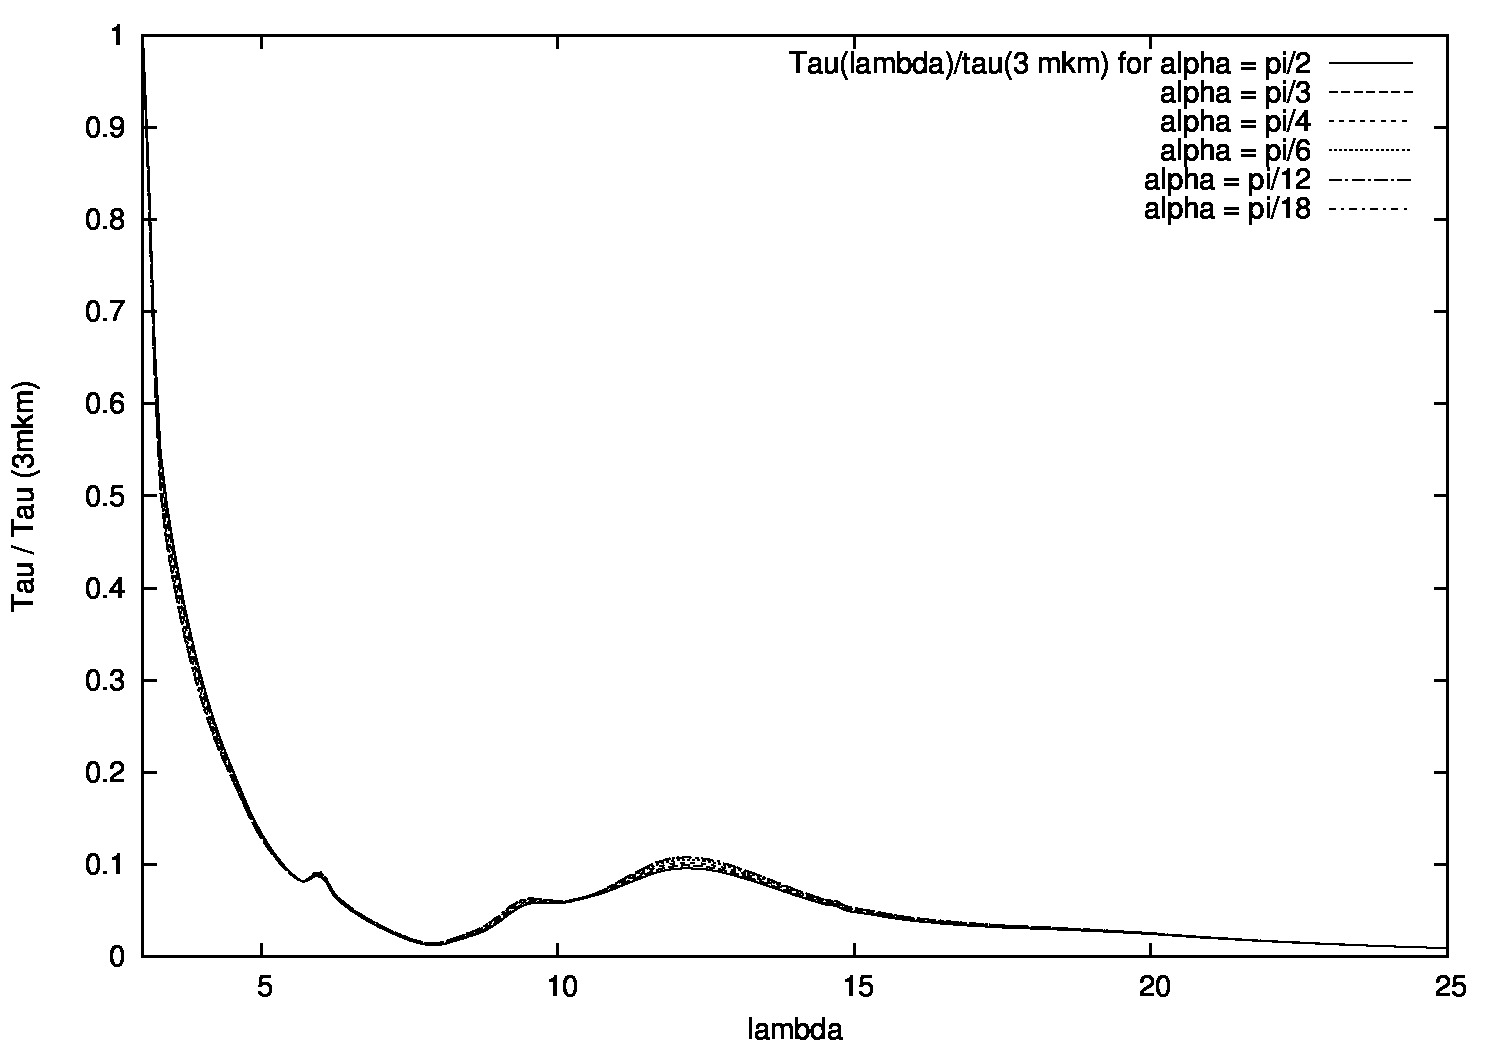
\includegraphics{../plots/tau-1-07.jpg}
 \caption{$\tau(\lambda)/\tau(3\mu m)$ }
\end{figure}

\begin{figure}[p]
 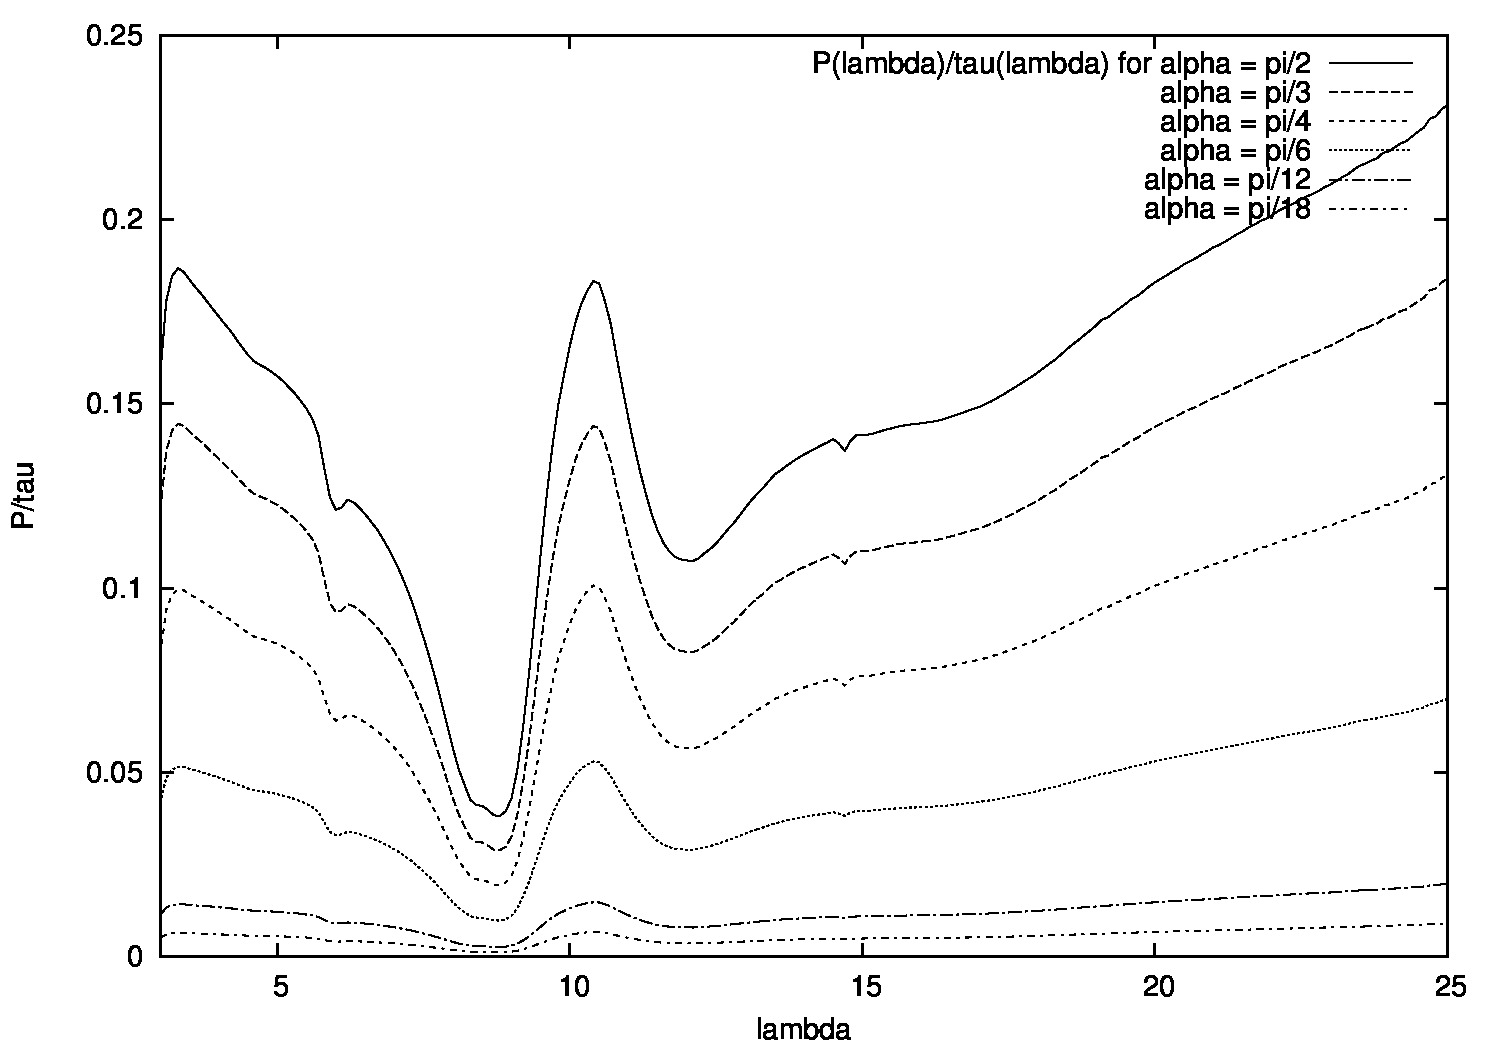
\includegraphics{../plots/P-to-tau-1-07.jpg}
 \caption{$P(\lambda)/\tau(\lambda)$ }
\end{figure}


\begin{figure}[p]
 $$a_{ice} = 1 \mu m,b_{ice} = 0.3 \mu m , a_{sil} = 0.1 \mu m , b_{sil} = 0.03  \mu m $$
 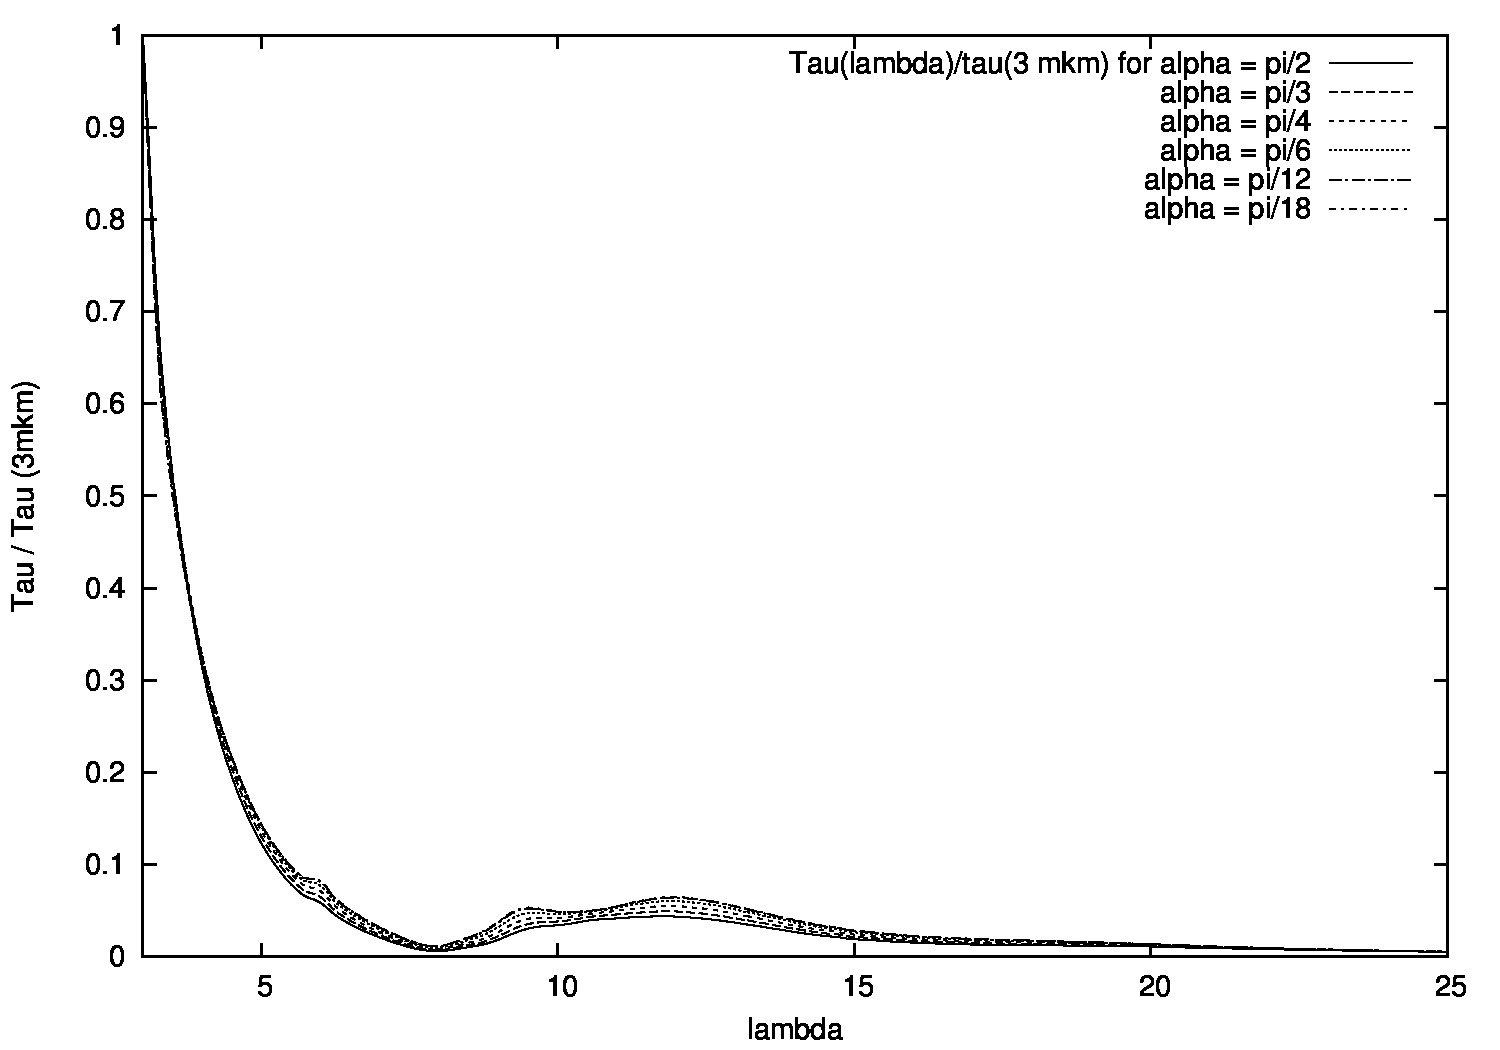
\includegraphics{../plots/tau-1-03.jpg}
 \caption{$\tau(\lambda)/\tau(3\mu m)$ }
\end{figure}

\begin{figure}[p]
 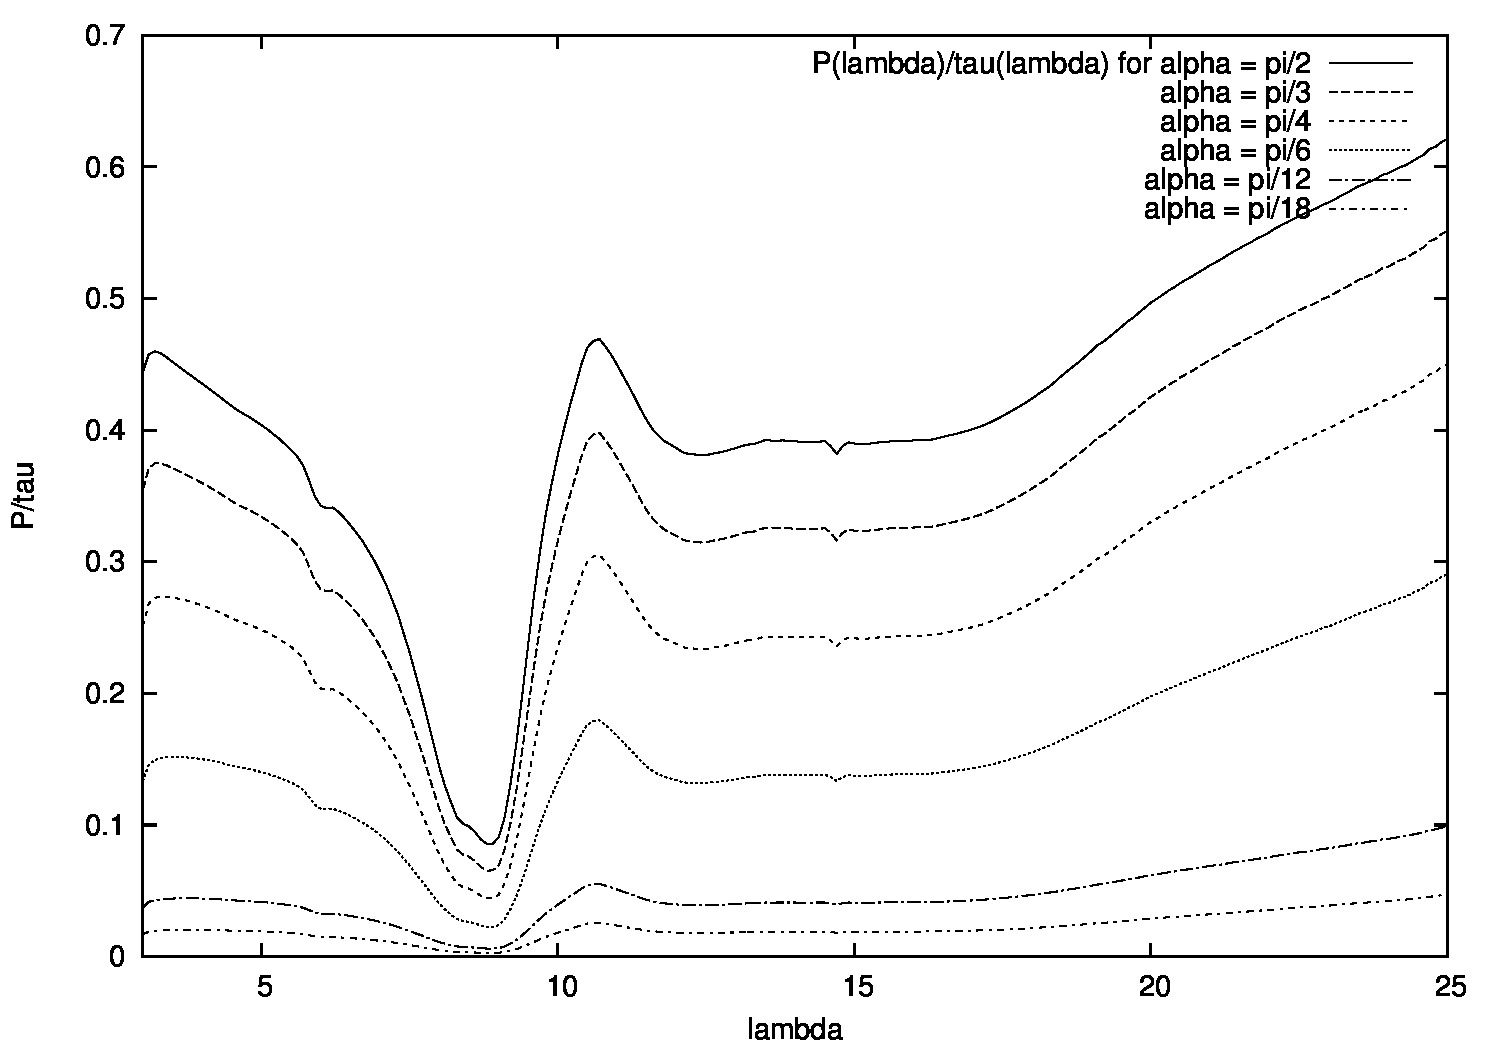
\includegraphics{../plots/P-to-tau-1-03.jpg}
 \caption{$P(\lambda)/\tau(\lambda)$ }
\end{figure}

\begin{figure}[p]
$$a_{ice} = 3 \mu m,b_{ice} = 0.1 \mu m , a_{sil} = 0.3 \mu m , b_{sil} = 0.01  \mu m $$
 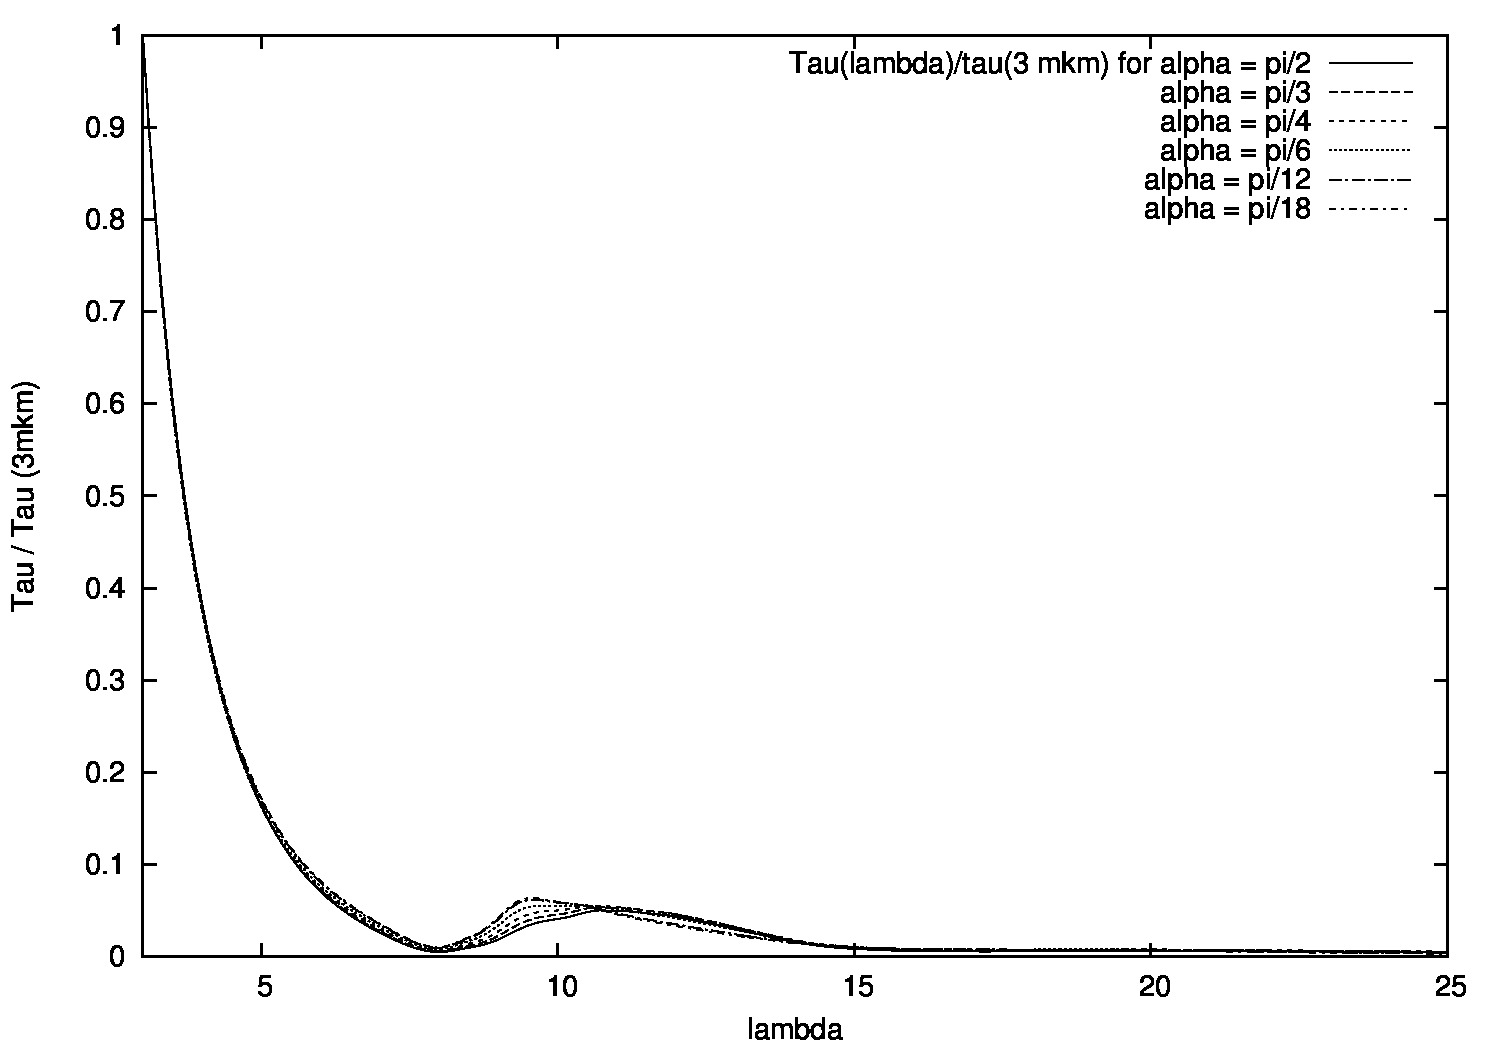
\includegraphics{../plots/tau-3-01.jpg}
 \caption{$\tau(\lambda)/\tau(3\mu m)$ }
\end{figure}

\begin{figure}[p]
 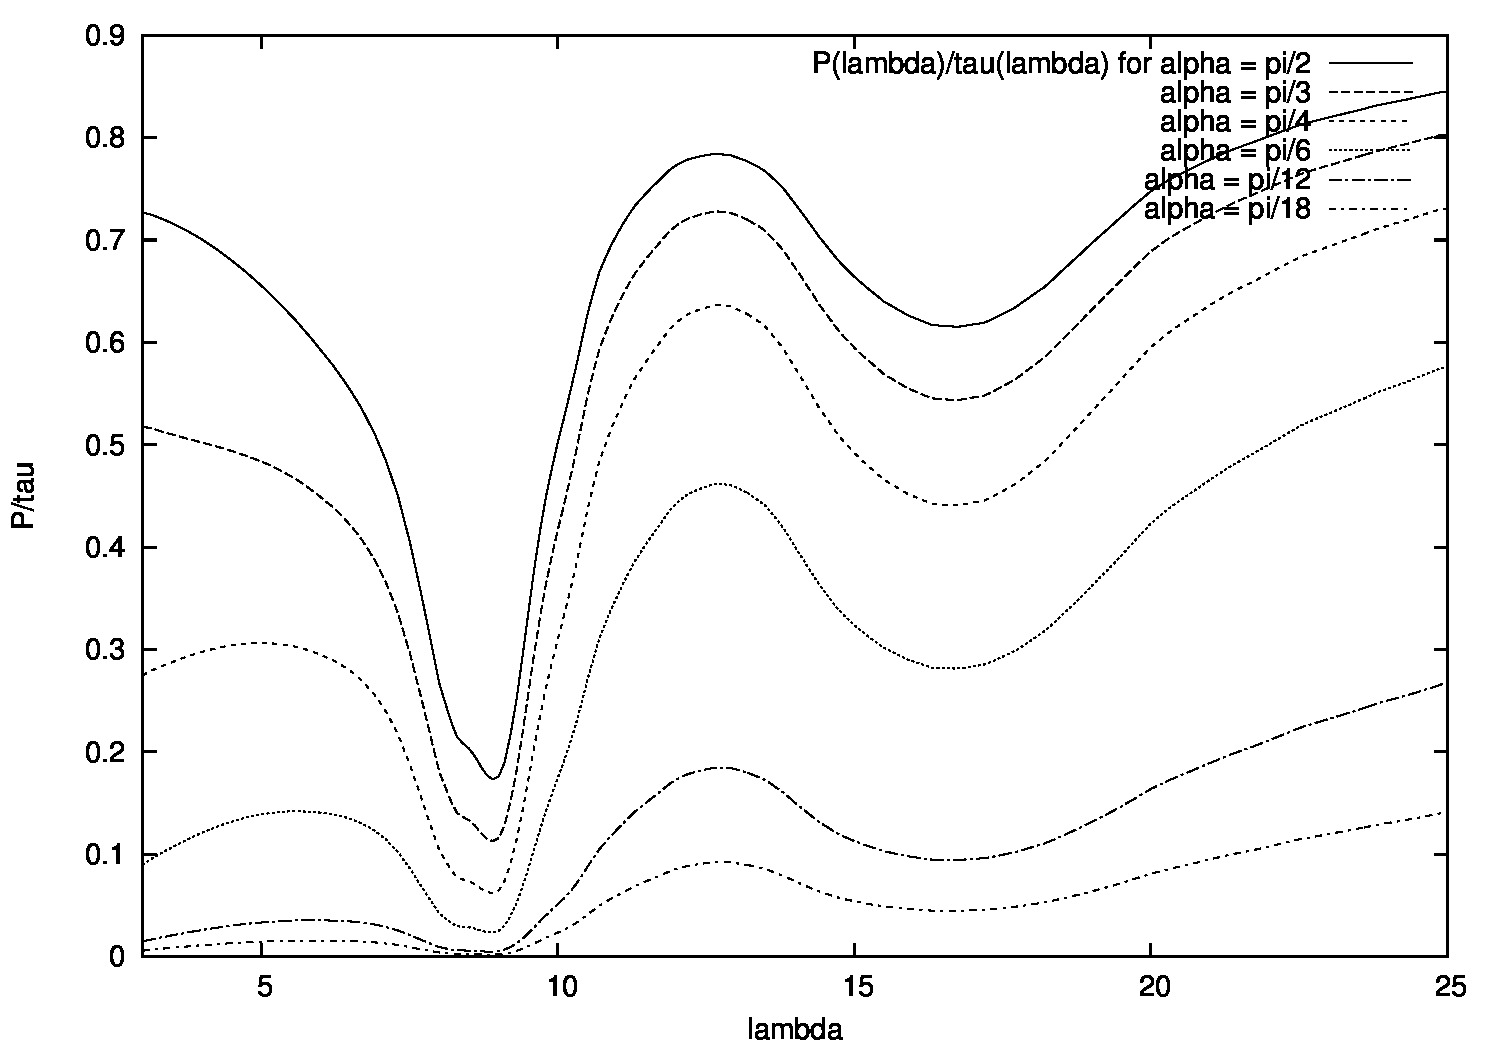
\includegraphics{../plots/P-to-tau-3-01.jpg}
 \caption{$P(\lambda)/\tau(\lambda)$ }
\end{figure}
  %% стилевой файл для оформления по ГОСТу
\bibliography{report}
\end{document}